\section{Einf"uhrung}
Vor der Planung des eigentlichen Programmsablauf, der Entwicklung der Algorithmen und der Implementierung des Programms und der GUI haben wir uns grundlegende Gedanken zur Aufteilung des Programms gemacht und folgendes Modell entwickelt.\\
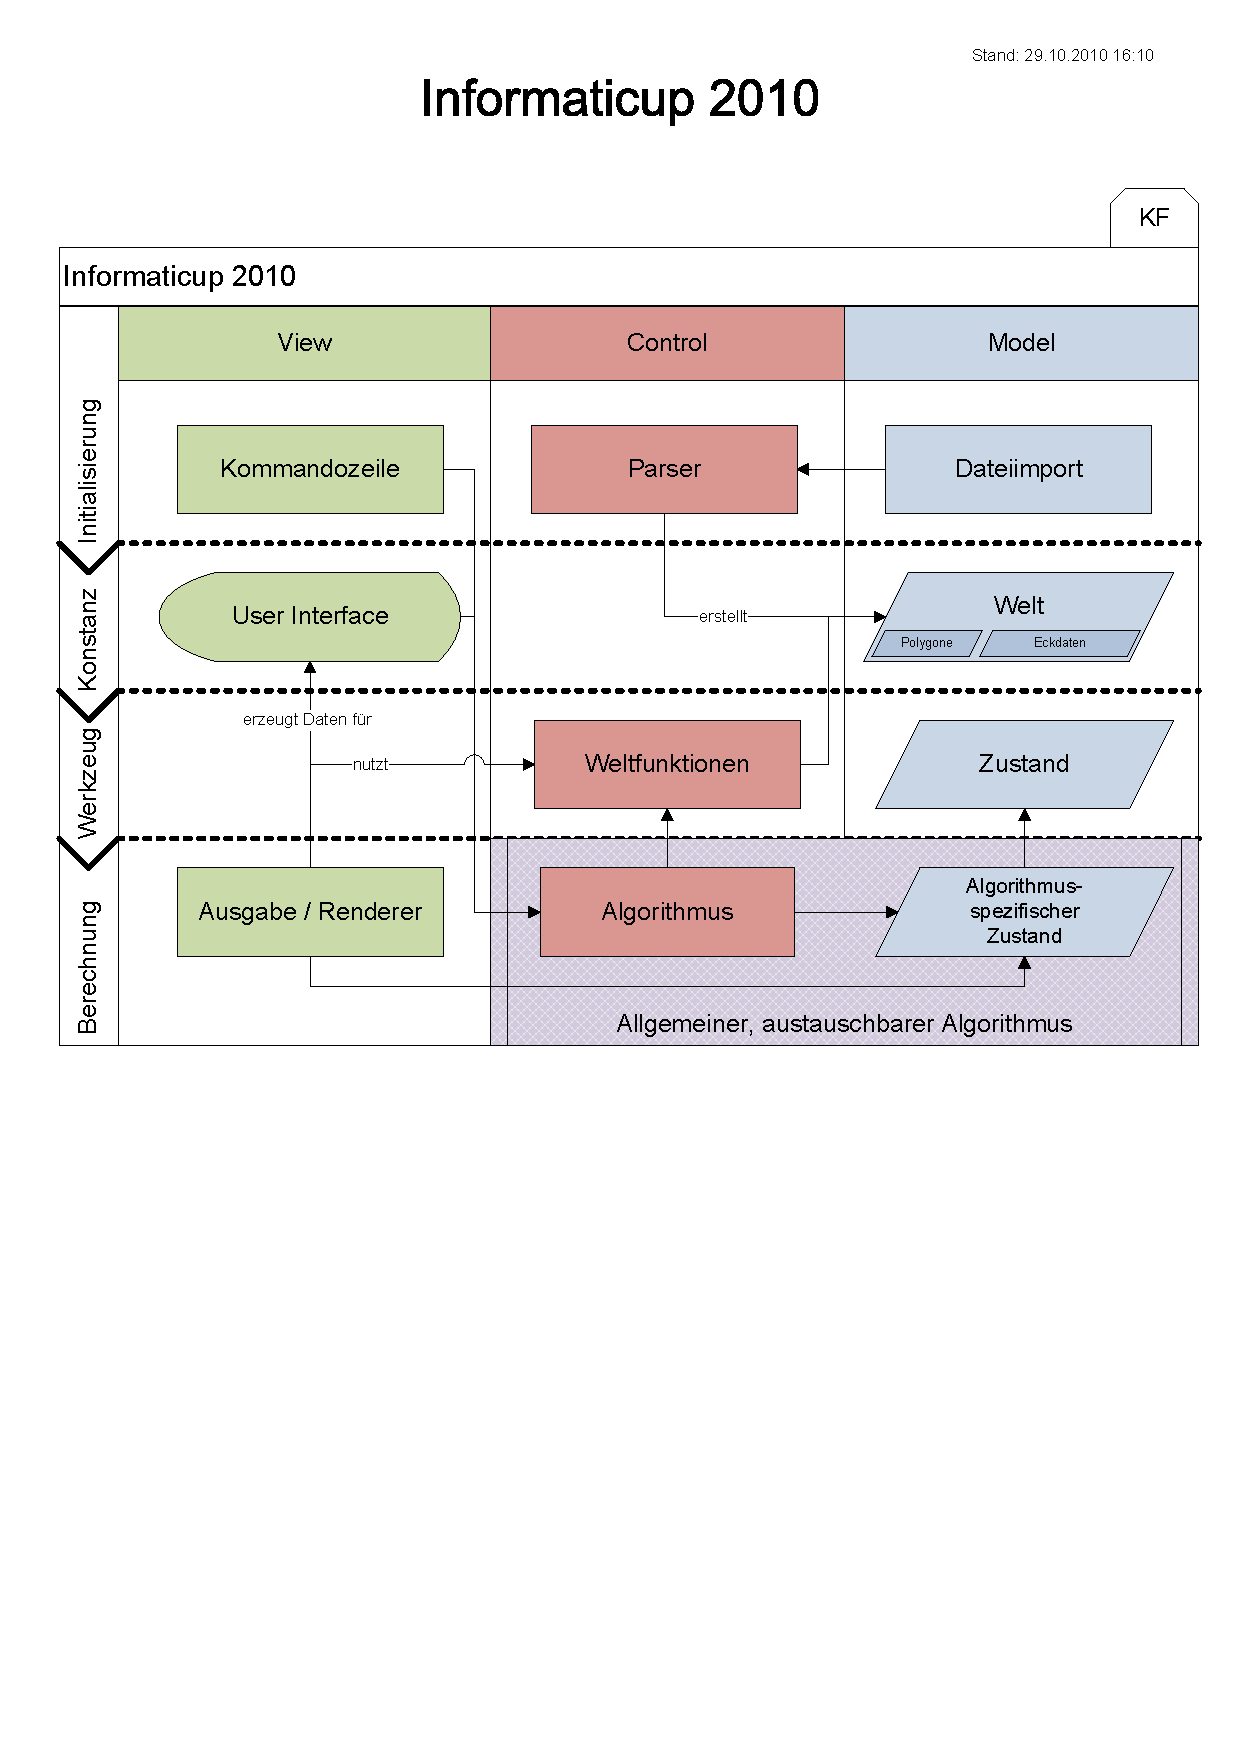
\includegraphics[width=1.0\textwidth]{scheme.pdf}
Dieses Modell entspricht nicht mehr dem aktuellem Stand, war jedoch Anfangs als ein grobes Konzept sehr hilfreich.\\
Zur Umsetzung unserer Ideen benutzten wir die NetBeans IDE unter Verwendung der Programmiersprache Java unter Windows. Unser Projekt ist sehr modular aufgebaut und in verschiedene Packages und Klassen unterteilt. Diese modulare und objektorientierte Programmentwicklung hatte insbesondere folgende Vorteile.
\begin{itemize}
\item \textbf{Teamf"ahigkeit:} Verschiedene Mitglieder eines Teams k"onnen gleichzeitig an verschiedenen Klassen/Teilen des Projekts arbeiten. Dies war besonders wichtig, weil drei Personen in Potsdam und eine Person in Regensburg am Projekt arbeitete. Als Versionsverwaltung setzten wir Subversion ein.
\item \textbf{Leichte Austauschbarkeit von Quelltext:} "Anderungen, Verbesserungen und neue Algorithmen k"onnen ohne gro"sen Aufwand implementiert werden.
\end{itemize}
Die Dokumentation wurde mit \LaTeX\ (TeX Live 2010) erstellt.